\documentclass[11pt]{article}
\usepackage[letterpaper,margin=1in]{geometry}
\usepackage{listings}
\usepackage{url}
\usepackage{hyperref}
\usepackage{textcomp}
\usepackage{graphicx}
\usepackage{underscore}
\usepackage{float}
\lstset{%
  basicstyle=\small\ttfamily,
  mathescape=true,
  upquote=true,
}

\usepackage{amsmath,amsbsy,amsfonts,amssymb,amsthm,color,dsfont,mleftright,commath}

\def\ddefloop#1{\ifx\ddefloop#1\else\ddef{#1}\expandafter\ddefloop\fi}

% \bbA, \bbB, ...
\def\ddef#1{\expandafter\def\csname bb#1\endcsname{\ensuremath{\mathbb{#1}}}}
\ddefloop ABCDEFGHIJKLMNOPQRSTUVWXYZ\ddefloop

% \cA, \cB, ...
\def\ddef#1{\expandafter\def\csname c#1\endcsname{\ensuremath{\mathcal{#1}}}}
\ddefloop ABCDEFGHIJKLMNOPQRSTUVWXYZ\ddefloop

% \vA, \vB, ..., \va, \vb, ...
\def\ddef#1{\expandafter\def\csname v#1\endcsname{\ensuremath{\boldsymbol{#1}}}}
\ddefloop ABCDEFGHIJKLMNOPQRSTUVWXYZabcdefghijklmnopqrstuvwxyz\ddefloop

% \valpha, \vbeta, ...,  \vGamma, \vDelta, ...,
\def\ddef#1{\expandafter\def\csname v#1\endcsname{\ensuremath{\boldsymbol{\csname #1\endcsname}}}}
\ddefloop {alpha}{beta}{gamma}{delta}{epsilon}{varepsilon}{zeta}{eta}{theta}{vartheta}{iota}{kappa}{lambda}{mu}{nu}{xi}{pi}{varpi}{rho}{varrho}{sigma}{varsigma}{tau}{upsilon}{phi}{varphi}{chi}{psi}{omega}{Gamma}{Delta}{Theta}{Lambda}{Xi}{Pi}{Sigma}{varSigma}{Upsilon}{Phi}{Psi}{Omega}{ell}\ddefloop

\newcommand\braces[1]{\{#1\}}

\theoremstyle{definition}
\newtheorem{problem}{Problem}
\newenvironment{solution}{\noindent\emph{Solution.}}{\hfill$\square$}

%-------------------------------------------------------------------------------

\title{COMS 4771 Spring 2017 Homework 4}
\author{Jin Tack Lim, jl4312
  }
\date{%
  }

\begin{document}
\maketitle


%-------------------------------------------------------------------------------

Problem 1.

(a) 

Consider the case in Figure~\ref{fig:one-rest}. There are three cases: C1, C2 and C3. Using
'one vs. rest', we can draw three lines, which classify a sample to either a
specific class or other classes. The whole space is divided into seven regions.
Out of seven, there are three regions that is classified to a specific class
clearly: R2 is C2, R4 is C3 and R6 is C1.  However there is a region that
doesn't fit into any class: R1. Also, there are regions that are classified
into multiple classes: R3, R5, R7.

So, this example showed that 'one vs. rest' has some drawbacks.

\begin{figure}[h]
  \centering
  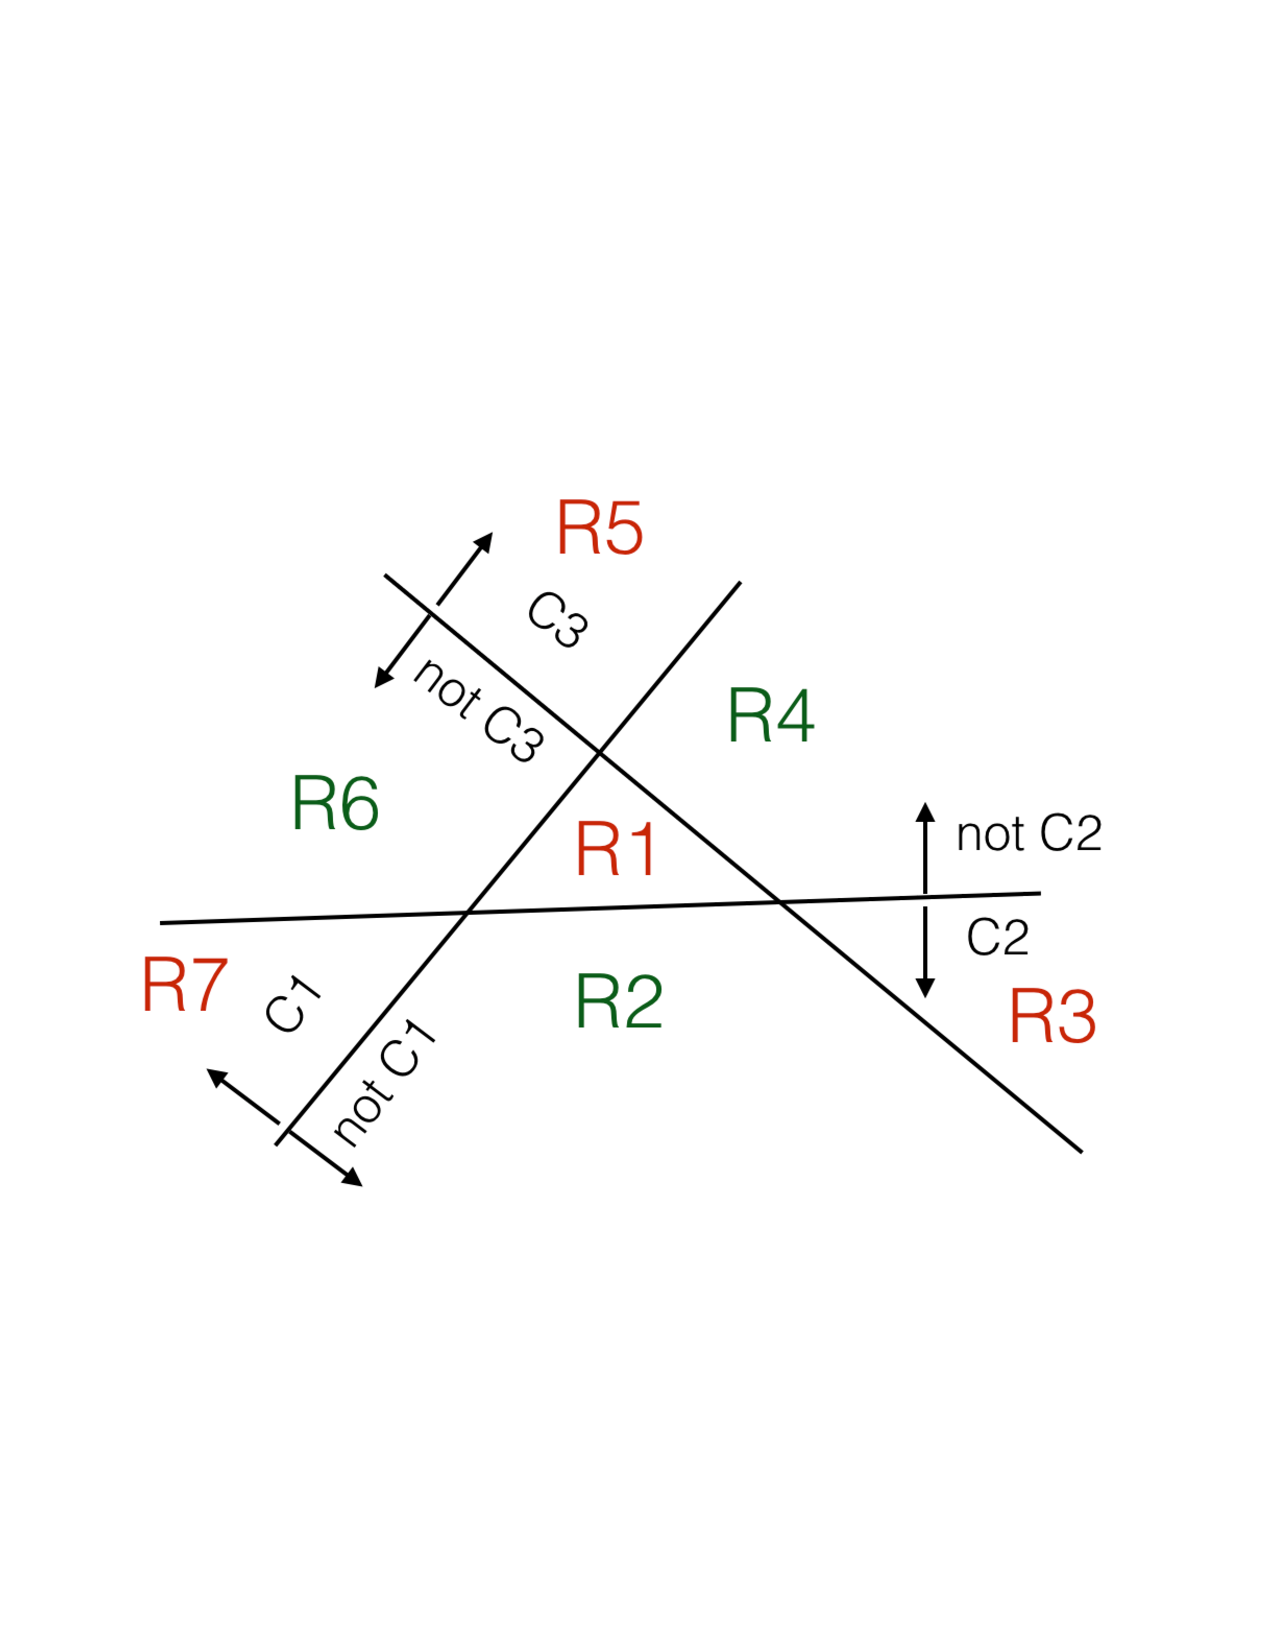
\includegraphics[width=10cm]{one-rest}
  \caption{One vs. rest}
  \label{fig:one-rest}
\end{figure}

\pagebreak

(b)

Consider the case in Figure~\ref{fig:one-one}. There are three cases: C1, C2 and C3. Using
'one vs. one', we can draw three lines (3*2/2), which classify a sample to one
of two classes for each pair of classes.  The whole space is divided into seven
regions.  Out of seven, six regions are clearly classified into a specific
class: R6 and R7 are C1, R2 and R3 are C2, R4 and R5 are C3.  However R1 can't
be classified because there is no single winner: 1 vote for each classes.

So, this example showed that 'one vs. one' also has some drawbacks.

\begin{figure}[h]
  \centering
  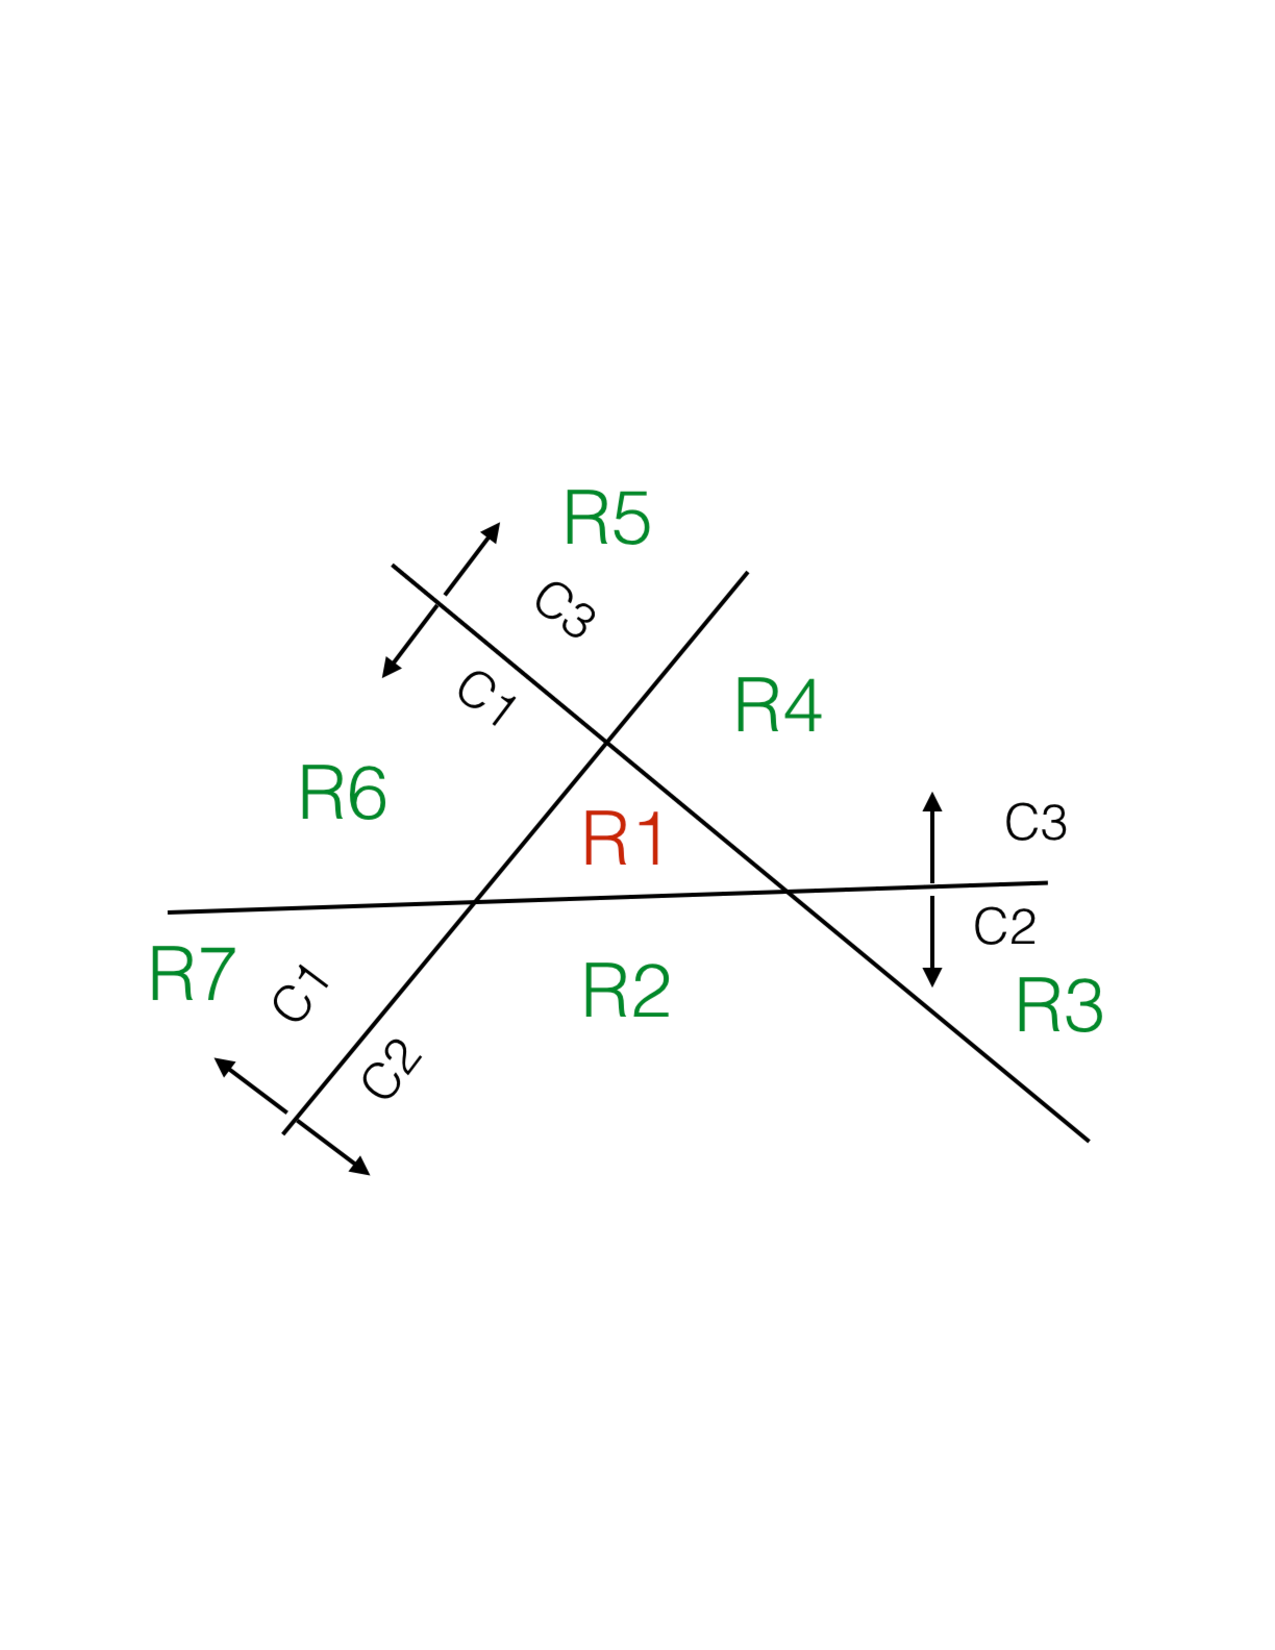
\includegraphics[width=10cm]{one-one}
  \caption{One vs. One}
  \label{fig:one-one}
\end{figure}

\pagebreak

(c)

1. The primal and quadratic problem:

\begin{equation*}
\arg \min_{w,b} \frac{1}{2} \sum_{m=1}^{k} \norm{w}^2 + C \sum_{i=1}^{N}\xi_i \quad \text{such that}
\end{equation*}
\begin{equation*}
\quad y_i (w_m^T x_i + b) -1 + \xi_i \ge 0 \quad \text{for each dimension m (from 1 to k)}
\end{equation*}

With Lagrange $\alpha$:

\begin{equation*}
\arg \min_{w,b} \frac{1}{2} \sum_{m=1}^{k} \norm{w}^2 + C \sum_{i=1}^{N}\xi_i
- \sum_{i=1}^{N}\sum_{m=1}^{k}\alpha_{i}^{m}(y_i(w_m^T x_i + b) -1 + \xi_i)
- \sum_{i=1}^{N}\beta_i\xi_i
\end{equation*}
all $\alpha$ and $\beta \ge 0$

\bigskip


2. The dual problem:
%We first define a new notation $A_i$
%\begin{equation*}
%A_i = \sum_{m=1}^{k} \alpha_{i}^{m}
%\end{equation*}

\begin{equation*}
\arg \max_\alpha \sum_{i,m} \alpha_{i}^{m} - \frac{1}{2} \sum_{i,j,m} \alpha_{i}^{m} \alpha_{j}^{m} y_i y_j x_i^T x_j
\end{equation*}
\begin{equation*}
\text{subject to} \quad 0 \le \sum_{m}\alpha_{i}^{m} \le C \quad \text{and} \sum_{i=1}^{N}\sum_{m=1}^{k} \alpha_{i}^{m} y_i =0 
\end{equation*}

\pagebreak

Problem 2.

\bigskip

(a)
\begin{equation*}
\sum_{i=1}^{k}p_i \log p_i
\end{equation*}


This is the Entropy without the negative sign.

This is how I got the expectation.

(1) When the value of $y_i$ is $j$, then its contribution is $\log p_j$.

(2) The probability that $y_i$ becomes $j$ is $p_j$.

(3) Therefore the expectation is the sum of $p_j \log p_j$ over all possible j (1,...,k)

\bigskip
(b)

\begin{equation*}
\sum_{i=1}^{k}p_i \log q_i
\end{equation*}

\bigskip

\pagebreak

Problem 3.

\bigskip
a) The marginal distribution is the binomial distribution. More specifically, the probablity of being weight k is
\begin{equation*}
\binom{n}{k}  \Big(\frac{1}{n}\Big)^k \Big({\frac {n-1}{n}}\Big)^{n-k}
\end{equation*}

The correlation of each weight is, intuitively, if one of the weight is k, then the other weight should be equal to or less than n-k. In other words, the distribution of the former is ~Bin(n, p) and the latter is ~Bin(n-k, p)

\bigskip
b)
This is a hard problem, so I read some papers[1][2][3] and borrowed their idea.

Step 1. Show that the error $\epsilon$ from the booster(i.e. Adaboost) is bounded by the product of $Z_t$.
\begin{equation*}
\epsilon = \frac{1}{m} * {\text{number of mispredicted points}} \le \prod_{t} Z_t
\end{equation*}

Step 2. Show that the product of Z is bounded by the expression with T and $\gamma$.
\begin{equation*}
\prod_{t} Z_t \le \exp(-2T\gamma^2)
\end{equation*}

Step 3. Device the given form in the problem from the step 1 and 2.
\begin{equation*}
T = - \frac{\gamma^2}{C\log \epsilon}
\end{equation*}

\bigskip
Here are the detailed steps.

Step 1.

\begin{equation*}
\epsilon = \frac{1}{m} * {\text{number of mispredicted points}} \le 
\frac{1}{m} \sum_{i} \exp(-y_if(x_i)) =
\prod_{t} Z_t
\end{equation*}

The inequality comes from the fact that $\exp(-y_if(x_i)) \ge 1$ if the data point is mispredicted. The equality comes by unraveling the recursive definition of $D_t$

Step 2.

This step is way too much complicated for me to digest.

Step 3.

By combining the result from step 1 and step 2, we can derive this form.
C in this case is $\frac{1}{2}$

\begin{equation*}
T \le - \frac {\log \epsilon}{2\gamma^2}
\end{equation*}

\bigskip
References

[1] A Decision-Theoretic Generalization of On-Line Learning and an Application to Boosting, Freund and Schapire, 
http://www.face-rec.org/algorithms/Boosting-Ensemble/decision-theoretic_generalization.pdf

[2] Improved Boosting Algorithms
Using Confidence-rated Predictions, Schapire and Singer, http://web.cs.iastate.edu/~honavar/singer99improved.pdf

[3] The Boosting Approach to Machine Learning An Overview, Schapire, https://www.cs.princeton.edu/courses/archive/spring07/cos424/papers/boosting-survey.pdf
\end{document}
